The following chapter describes the design behind the assignment of the missions to the resources. The system considers \textit{eight} resources, each of one is the composition of human operator and forklift. The orders are known at the beginning of the startup and they are assigned progressively, keeping every mission of a singular order attached to their resource.

The 

La politica organizza le decisioni mediante interventi globali di batching.
Il parametro $x$ definisce il
numero di nuove missioni da aggiungere a ogni refill e, nella configurazione
adottata, il numero di completamenti globali che attiva l'intervento
successivo. Le nuove missioni si aggiungono al lavoro eventualmente residuo:
$x$ non costituisce una capienza massima dell'insieme delle missioni ammesse.

La simulazione conserva lo stato delle risorse durante ciascuna
riassegnazione. Una risorsa con una missione in esecuzione mantiene il
percorso e il completamento programmato; una risorsa che ha esaurito la
propria coda può ricevere nuovo lavoro a partire dall'istante in cui l'ha
terminata. L'istante della decisione globale viene pertanto distinto dagli
istanti locali di inserimento delle nuove missioni. Il metodo costruisce
una pianificazione offline, nella quale è possibile completare
retroattivamente la timeline delle singole risorse.

L'esecuzione è governata da Colored Timed Petri Net (CTPN), che rappresenta le precedenze e la
riserva della risorsa. Il planner A* determina percorsi e durate delle
missioni avviate. La stima euclidea è utilizzata esclusivamente per fissare
le deadline degli ordini e valutarne il rispetto a posteriori; non
interviene nell'assegnazione, nel refill o nell'abilitazione degli avvii.

Nel modello discusso si assume che i dati preparati definiscano missioni
eseguibili e che tutte le missioni ammesse vengano portate a termine. 

\section{Ordini, missioni e risorse}
\label{sec:progetto-modello}

Siano $\mathcal O=\{o_1,\ldots,o_N\}$ l'insieme degli ordini e
$\mathcal R=\{1,\ldots,R\}$ quello delle risorse, con $R=8$ nella
configurazione di riferimento. Ogni ordine $o$ comprende un insieme di
missioni $\mathcal M_o$, di cardinalità $n_o=|\mathcal M_o|$.
Una missione descrive una movimentazione da un punto di prelievo FROM a un
punto di destinazione TO ed è caratterizzata da un codice, una priorità e
un'associazione all'ordine.

Ogni riga del dataset riceve anche un identificativo univoco di occorrenza.
Due missioni con lo stesso codice commerciale rimangono quindi attività
distinte. Una missione priva di identificativo d'ordine viene trattata come
un ordine autonomo, senza accorpare tra loro tutte le righe prive di tale
informazione.

Si indica con $\mathcal M_o^{\mathrm{adm}}$ l'insieme delle missioni
dell'ordine considerate dopo la preparazione dei dati. Il completamento
descritto nel seguito è riferito a tale insieme. La preparazione verifica
le informazioni necessarie e normalizza le coordinate prima
dell'assegnazione; le eventuali righe non ammesse rimangono esterne alla
rete operativa.

\begin{nota}
	Uno script Python divide i dati aziendali per giorno lavorativo. Ogni
	ordine resta interamente nello stesso lotto. Gli ordini del giorno sono
	noti prima di avviare la simulazione.
\end{nota}

\subsection{Vincolo di assegnazione ordine--risorsa}

Indicando con $r(o)$ la risorsa proprietaria dell'ordine, si impone
\begin{equation}
	r(m)=r(o),\qquad \forall m\in\mathcal M_o^{\mathrm{adm}}.
\end{equation}
Il proprietario viene scelto quando la prima missione dell'ordine viene
accodata. L'associazione resta invariata anche quando l'ordine attraversa
più interventi di batching. L'indivisibilità riguarda l'assegnazione alla
risorsa: non impone di inserire tutte le missioni dell'ordine in un unico
blocco di ammissione.

Una risorsa può essere proprietaria di più ordini, ma ne esegue uno alla
volta. Dall'avvio di un ordine fino alla conclusione della sua sequenza,
il token rimane riservato a quell'ordine. Le sue missioni non vengono
intercalate con quelle di altri ordini.

\subsection{Priorità e precedenze interne}

A ogni missione $m$ è associata una priorità numerica $p_m$. La sequenza
interna dell'ordine è
\begin{equation}
	\pi_o=(m_{o,1},\ldots,m_{o,n_o^{\mathrm{adm}}}),\qquad
	p_{m_{o,i}}\geq p_{m_{o,i+1}},
\end{equation}
dove $n_o^{\mathrm{adm}}=|\mathcal M_o^{\mathrm{adm}}|$.
A parità di priorità si mantiene l'ordine di ingresso; una priorità
mancante assume il valore convenzionale unitario.

Questa regola riguarda soltanto le missioni dello stesso ordine. I nuovi
ordini compatibili vengono considerati secondo la loro prima comparsa nel
dataset, senza ordinamenti per numero di missioni, durata prevista,
distanza o deadline. Le missioni residue di ordini già assegnati alla
risorsa hanno precedenza sull'apertura di nuovi ordini.

\section{Politica di assegnazione ordini}
\label{sec:progetto-assegnazione}

La politica applica i vincoli di compatibilità e assegnazione univoca
introdotti nella Sezione~\ref{sec:theory-eligibility}. Distingue
l'ammissione di nuovo lavoro dal dispatching delle missioni già in coda,
secondo la Sezione~\ref{sec:theory-batch-queues}. Lo scheduler stabilisce
quali attività aggiungere mentre la CTPN stabilisce quando tali attività possono
iniziare.

\subsection{Compatibilità dell'intero ordine}

Sia $\mathcal R_m\subseteq\mathcal R$ l'insieme delle risorse compatibili
con la missione $m$. Per l'ordine si considera
\begin{equation}
	\mathcal R_o=\bigcap_{m\in\mathcal M_o^{\mathrm{adm}}}\mathcal R_m.
\end{equation}
Per il problema corrente assume $\mathcal R_o\neq\varnothing$ per ogni
ordine. Il proprietario viene scelto in questo insieme, garantendo che
possa eseguire l'intera sequenza. L'associazione viene fissata dalla prima ammissione e
conservata nei refill successivi.

\subsection{Blocco globale e refill additivo}

Sia $k$ l'indice dell'intervento di batching. Si distinguono:
\begin{itemize}
	\item $\mathcal A_k^{-}$, le missioni già ammesse e non ancora
	completate prima del refill, comprendenti attese ed esecuzioni;
	\item $\mathcal N_k$, le nuove missioni inserite durante il refill;
	\item $\mathcal A_k^{+}$, il lavoro ammesso dopo l'assegnazione.
\end{itemize}
Le missioni nuove sono distinte dai residui e valgono
\begin{equation}
	\mathcal A_k^{+}=\mathcal A_k^{-}\cup\mathcal N_k,
	\qquad \mathcal A_k^{-}\cap\mathcal N_k=\varnothing,
	\label{eq:refill-insiemi}
\end{equation}
\begin{equation}
	|\mathcal N_k|\leq x,\qquad
	|\mathcal A_k^{+}|=|\mathcal A_k^{-}|+|\mathcal N_k|.
	\label{eq:refill-additivo}
\end{equation}
Quando rimangono almeno $x$ missioni assegnabili, $|\mathcal N_k|=x$, queste verranno inserite nell'ultimo blocco di rifornimento per le risorse.
Le $x$ missioni costituiscono il totale globale da distribuire tra le
risorse, non una quantità assegnata a ciascuna risorsa. Il lavoro residuo non riduce la dimensione del nuovo blocco. 
\begin{example}[Mission admission set]
	Con sette missioni ancora ammesse e $x=20$, un refill completo porta il
	lavoro ammesso a ventisette missioni. L'ammissione non si basa su un numero
	di posti liberi rispetto a una capienza fissa.
\end{example}

Si indica con $C_k$ il numero di eventi di completamento registrati nel
passaggio di esecuzione successivo all'assegnazione $k$ mentre il contatore delle missioni completate viene
azzerato all'inizio del passaggio. Al raggiungimento di
\begin{equation}
	C_k=x
	\label{eq:trigger-refill}
\end{equation}
il motore sospende l'elaborazione prima di ulteriori avvii e, se rimane
lavoro da assegnare, richiama lo scheduler. L'esaurimento della coda di una sola risorsa
non attiva autonomamente un refill.

Il contatore riguarda i completamenti elaborati nel passaggio, anche
quando appartengono a missioni ammesse in precedenza. Non va identificato
con un conteggio effettuato soltanto tra due istanti globali della timeline
finale, poiché nuovi eventi possono essere inseriti retroattivamente.

\begin{nota}
	Con inizializzazione vuota, primo blocco di $x$ missioni e soglia pari a
	$x$ completamenti, il primo refill avviene quando quel blocco è interamente
	concluso. La conservazione del lavoro residuo è una proprietà della
	procedura, non implica che a ogni confine vi siano necessariamente
	missioni in esecuzione. A parità di blocco e soglia, in assenza di residui
	iniziali, questa stessa condizione si ripete nei passaggi successivi.
\end{nota}

\subsection{Distribuzione delle missioni tra le risorse}

I principi di list scheduling della
Sezione~\ref{sec:theory-list-scheduling} vengono applicati considerando il
numero di missioni già ammesse per ciascuna risorsa. Per ogni risorsa si
definisce
\begin{equation}
	q_r=|\{m\in\mathcal A:\ r(m)=r\}|,
\end{equation}
dove $\mathcal A$ è l'insieme delle missioni ammesse ma non ancora
completate. Il conteggio include quindi sia la missione eventualmente in
esecuzione sia quelle presenti in coda.

Le risorse vengono considerate a partire da quella con il valore di $q_r$
più basso, così da favorire quelle che hanno meno missioni già assegnate.
In caso di parità, viene data precedenza alla risorsa che dispone di meno
ordini compatibili ancora non assegnati. Se una risorsa possiede già un
ordine con missioni ancora da accodare, tale condizione le conferisce
priorità. Gli eventuali ulteriori pareggi sono risolti in base all'indice
della risorsa. Il numero di ordini compatibili viene determinato all'inizio
dell'intervento, mentre $q_r$ viene aggiornato dopo ogni nuova ammissione.

Una volta scelta la risorsa, la missione da ammettere viene individuata
secondo due regole:
\begin{enumerate}
	\item Se esistono missioni ancora pendenti appartenenti a un ordine già
	assegnato alla risorsa, viene scelta la prima disponibile, nel rispetto
	delle precedenze interne all'ordine;
	\item In assenza di missioni proprie da accodare, viene selezionato il
	primo ordine compatibile ancora non assegnato, secondo l'ordine di
	ingresso, e ne viene ammessa la prima missione pendente.
\end{enumerate}
Dopo ogni inserimento il valore di $q_r$ viene aggiornato e la procedura
prosegue fino al completamento del nuovo blocco o all'esaurimento del
lavoro disponibile. Le missioni già presenti in coda mantengono comunque
la precedenza rispetto a quelle aggiunte successivamente.

Il criterio mira quindi a distribuire tra le risorse il numero di missioni
ammesse, senza utilizzare una stima della loro durata. Di conseguenza, non
garantisce né carichi temporali uguali né che tutte le risorse rimangano
continuamente occupate. Il tempo di lavoro effettivo dipende infatti dai
percorsi delle missioni e dalle caratteristiche degli ordini assegnati.

\subsection{Riferimento temporale nominale}

Il tempo nominale per missione $\overline{\tau}=180\,\mathrm{s}$ consente
di definire il riferimento
\begin{equation}
	H=\frac{x\,\overline{\tau}}{R}.
	\label{eq:budget_temporale_batch}
\end{equation}
Indicando con $T_k$ l'istante della decisione globale $k$, si associa al
passaggio la scadenza nominale
\begin{equation}
	D_k=T_k+H.
\end{equation}
Questo riferimento è utilizzato soltanto nel report. Non dimensiona le
code, non determina il refill e non interrompe l'esecuzione. La durata
delle missioni viene ricavata da A*. \begin{comment}
	mentre le deadline dei singoli ordini
	seguono il modello euclideo della
	Sezione~\ref{sec:stima-deadline-euclidea}.
\end{comment}


\section{CTPN per la riserva della risorsa}
\label{sec:progetto-ctpn}

Il modello applica la rappresentazione colorata temporizzata introdotta
nella Sezione~\ref{sec:theory-ctpn}, specializzando la riserva del token
alla sequenza di missioni di un ordine.

\begin{figure}[H]
	\centering
	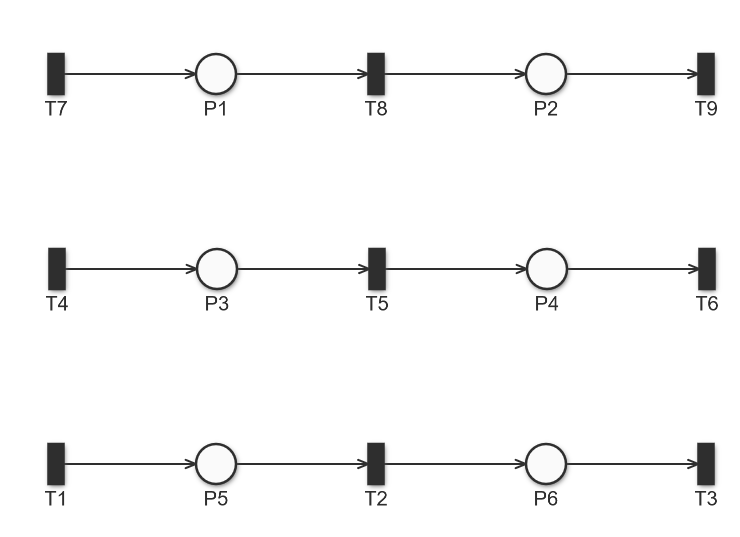
\includegraphics[width=0.7\linewidth]{imgs/Cap2_teoria/NEW_PN2_VECCHIA_MISSIONI}
	\caption{Schema di riferimento della modellazione precedente delle alternative di risorsa per una singola missione.}
	\label{fig:pn2vecchiamissioni}
\end{figure}


\noindent La Figura~\ref{fig:pn2vecchiamissioni} richiama lo schema precedente,
organizzato intorno alle alternative di risorsa per una singola missione.
Nella soluzione adottata lo scheduler assegna la risorsa all'intero ordine
quando accoda la prima missione. La rete
non seleziona un nuovo proprietario
per ogni missione, ma utilizza il colore della risorsa già assegnata.


Ciascuna missione mantiene una sottorete con tre transizioni e due posti
interni. Le tre fasi rappresentano l'avvio, il completamento temporizzato
e il passaggio alla missione seguente oppure il rilascio della risorsa.
Le sottoreti dello stesso ordine vengono collegate in sequenza secondo
le priorità interne.

\subsection{Intra-order links}
Tra due missioni consecutive viene inserito un posto di collegamento che
riceve il token dalla transizione finale della precedente e lo rende
disponibile alla transizione iniziale della successiva. Il token conserva
il colore della risorsa assegnata. Il posto di collegamento rappresenta
quindi sia la precedenza sia il mantenimento della riserva operativa.

La Figura~\ref{fig:pn1nuovamissioni} mostra una sequenza di tre missioni;
i posti $P7$ e $P8$ collegano le rispettive sottoreti. Lo schema evidenzia
le precedenze e va letto insieme al vincolo sul colore della risorsa.

\begin{figure}[H]
	\centering
	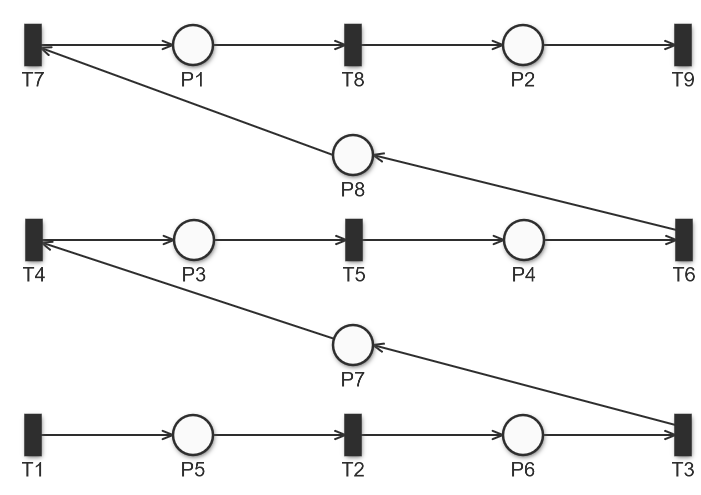
\includegraphics[width=0.7\linewidth]{imgs/Cap2_teoria/NEW_PN1_NUOVA_MISSIONI}
	\caption{Collegamento tra tre missioni dello stesso ordine mediante posti di precedenza. Il token della risorsa viene trasferito lungo la sequenza senza essere restituito al posto comune tra missioni intermedie.}
	\label{fig:pn1nuovamissioni}
\end{figure}

Solo la prima missione dell'ordine preleva il token dal posto comune delle
risorse disponibili; solo l'ultima missione ammessa lo restituisce.
All'interno dell'ordine, la disponibilità necessaria all'avvio è rappresentata
dal token nel posto di collegamento: non occorre prelevare nuovamente una
risorsa libera dal posto comune.

Per ogni risorsa $r\in\mathcal R$ esiste esattamente un token di colore
$r$ nella rete operativa. La conservazione del token è espressa
dall'invariante di posto
\begin{equation}
	\sum_{p\in\mathcal P}M(p)(r)=1,
	\qquad \forall r\in\mathcal R,
\end{equation}
dove $M(p)(r)$ indica la molteplicità del colore $r$ nel posto $p$ e
$\mathcal P$ è l'insieme dei posti della rete. La marcatura determina le
transizioni abilitate, mentre l'associazione ordine--risorsa stabilisce
il colore che può partecipare al loro scatto.

\begin{nota}
	Per semplicità di rappresentazione, le reti di Petri mostrate nelle figure non sono CPN, bensì PN. Questo perché ciascuna figura rappresenta un singolo ramo della rete, percorso da token appartenenti a un unico colore, consentendo così una rappresentazione grafica semplificata.
\end{nota}

\subsection{Conservazione della riserva durante il refill}

La sospensione per il batching non costituisce una transizione di rilascio.
Il token di una risorsa in esecuzione rimane nel posto di lavoro della
missione corrente. Anche il token che attende la missione successiva dello
stesso ordine rimane nel posto di collegamento, senza tornare al posto
comune. La risorsa viene rilasciata soltanto alla conclusione dell'ordine.

Il refill modifica le ammissioni e, per i nuovi ordini, l'associazione alla
risorsa. Non ricostruisce la rete, non reinizializza la marcatura e non
ricalcola il percorso di una missione già avviata. L'avvio richiede
congiuntamente l'ammissione della missione e l'abilitazione della relativa
transizione nella CTPN.

\section{Continuità dello stato tra batch}
\label{sec:progetto-tempo}

\subsection{Stato persistente e risorse in esecuzione}

Tra due interventi si conservano la \textbf{marcatura}, i \textbf{proprietari degli ordini},
le \textbf{code residue}, le \textbf{posizioni raggiunte}, i \textbf{percorsi delle missioni avviate}
e i \textbf{relativi istanti di inizio} e \textbf{fine programmata}. Vengono conservati anche
la cronologia dei completamenti e i valori delle deadline già fissate.
Il contatore $C_k$ viene invece azzerato per il nuovo passaggio.

L'indicatore \textit{in work} rappresenta il numero di risorse con una
missione avviata e non ancora completata nello stato sospeso. Non comprende
le missioni soltanto in attesa. Poiché ogni risorsa può eseguire una sola
missione alla volta, tale indicatore coincide con il numero di missioni
attualmente in esecuzione.

\subsection{Eventi di esecuzione e soglia globale}

L'avanzamento riprende il principio della Scheduled Event List descritto
nella Sezione~\ref{sec:theory-sel}. Per una missione $m$ avviata
all'istante $s_m$ e di durata $\tau_m$, il completamento è programmato a
\begin{equation}
	c_m=s_m+\tau_m.
\end{equation}
Il motore elabora gli eventi concorrenti e incrementa $C_k$ a ogni
completamento. Finché la soglia non è raggiunta, una risorsa può avviare la
successiva missione ammessa e abilitata, senza richiamare lo scheduler.

Quando $C_k=x$, il motore conserva lo stato prima di altri avvii. Gli altri
eventi eventualmente programmati allo stesso istante vengono elaborati
nel passaggio successivo, senza introdurre un ritardo fisico. Questa
convenzione mantiene esatto il conteggio dei completamenti del passaggio.

Se non rimangono nuove missioni da ammettere, il motore continua a eseguire
il lavoro già assegnato. La simulazione termina quando tutte le missioni
ammesse dopo la preparazione sono completate. L'ultimo passaggio può
contenere meno di $x$ completamenti quando il lavoro residuo è inferiore
alla soglia.

\subsection{Decisione globale e ripartenza locale}

Si distingue l'istante $T_k$ della decisione globale dal cursore temporale
$\theta$ usato per elaborare gli eventi. Le decisioni globali mantengono
una sequenza non decrescente; il cursore può invece tornare a un istante
precedente per inserire lavoro sulla timeline di una risorsa.

Per una risorsa che ha esaurito la propria coda, sia $f_{r,k}$ il suo ultimo
istante di completamento noto prima del refill. Il nuovo lavoro può essere
inserito a partire da
\begin{equation}
	a_{r,k}=f_{r,k},
	\label{eq:ripartenza-locale}
\end{equation}
anche quando $a_{r,k}<T_k$. Per una risorsa mai impiegata, la frontiera
iniziale è posta a zero. Se la risorsa conserva lavoro in coda o in
esecuzione, le aggiunte rispettano tale lavoro e non ne anticipano
l'esecuzione.


\begin{example}[Back-to-the-Future assignment]
	Una risorsa che ha terminato la coda a $80\,\mathrm{s}$ può
	ricevere il blocco successivo a partire da tale istante anche se la
	decisione globale viene registrata a $120\,\mathrm{s}$. Il nuovo lavoro
	viene inserito nell'intervallo temporale precedentemente rimasto libero.
\end{example}

\noindent Il ritorno temporale non annulla gli eventi già consolidati sulle altre
risorse. Ciascuna mantiene la propria frontiera: non si avviano due
missioni contemporaneamente sulla stessa risorsa e non si modifica una
missione già in work. In particolare, il suo istante di completamento
$c_m$ rimane quello definito all'avvio.

Gli eventi aggiunti nel passato appartengono al nuovo passaggio di
elaborazione. Se il cursore raggiunge il target in un istante
$\theta_k^{\mathrm{stop}}$ precedente all'ultima decisione globale,
l'istante della decisione seguente è registrato come
\begin{equation}
	T_{k+1}=\max\{T_k,\theta_k^{\mathrm{stop}}\}.
	\label{eq:decisione-globale}
\end{equation}
Questa distinzione evita di attribuire a tutte le risorse un unico istante
di ripartenza e separa la sequenza delle decisioni dalla timeline finale.

\begin{nota}
	La procedura costruisce una pianificazione offline a partire da ordini
	noti. L'inserimento retroattivo completa la timeline simulata; non descrive
	un comando che un sistema fisico potrebbe eseguire nel passato. Le durate
	di calcolo del programma non vengono sommate ai tempi operativi simulati.
\end{nota}



\begin{comment}
	
	\subsection{Procedura di batching}
	
	La sequenza operativa può essere riassunta nei seguenti passi:
	\begin{enumerate}
		\item conservare tutte le missioni ammesse non ancora completate e lo
		stato delle risorse;
		\item aggiungere fino a $x$ nuove missioni, privilegiando le continuazioni
		degli ordini già assegnati e mantenendo l'ingresso per i nuovi ordini;
		\item per le risorse con coda esaurita, riprendere dalla rispettiva
		frontiera temporale; mantenere le esecuzioni delle altre risorse;
		\item elaborare le missioni ammesse tramite la CTPN e i percorsi A*,
		contando globalmente i completamenti;
		\item alla soglia $x$, sospendere l'elaborazione, registrare lo stato e
		ripetere il procedimento; terminare quando tutto il lavoro è concluso.
	\end{enumerate}
	
	
\end{comment}


\section{Stima euclidea delle deadline}
\label{sec:stima-deadline-euclidea}
\label{sec:stima-deadline-manhattan} % Alias per i riferimenti preesistenti.

Le scadenze applicano le definizioni della
Sezione~\ref{sec:theory-deadlines}. Sono indicatori osservativi, calcolati
per confrontare la previsione geometrica con i tempi di completamento.
Non vengono utilizzate per scegliere ordini, dimensionare code, assegnare
risorse o attivare refill.

La deadline dell'ordine viene fissata al primo avvio effettivo di una sua
missione. Non decorre dall'assegnazione del proprietario: l'attesa dovuta
agli ordini precedenti non consuma il budget del nuovo ordine. Tutte le
scadenze cumulative dell'ordine vengono congelate insieme e non vengono
ricalcolate durante i refill o la ripresa delle missioni successive.

\subsection{Sequenza e distanza stimata}

Si considera la sequenza $\pi_o$ delle missioni ammesse dell'ordine,
ordinata secondo le precedenze interne. Gli estremi $F_i$ e $T_i$ sono gli
indici della griglia corrispondenti a FROM e TO dopo normalizzazione e
arrotondamento. La previsione usa
\begin{equation}
	d_E(p,q)=\sqrt{(x_p-x_q)^2+(y_p-y_q)^2}.
	\label{eq:manhattan-distance} % Nome storico mantenuto per compatibilita.
\end{equation}
Sia $P_r$ la posizione della risorsa prima del primo avvio dell'ordine.
Si pone $Q_1=P_r$ e $Q_i=T_{i-1}$ per $i>1$; quando la risorsa non ha una
posizione precedente, si assume $Q_1=F_1$. La distanza prevista per ciascuna
missione è
\begin{equation}
	\widehat\ell_{o,i}=d_E(Q_i,F_i)+d_E(F_i,T_i).
	\label{eq:estimated-order-distance}
\end{equation}
Si includono così l'avvicinamento iniziale e gli spostamenti tra le
missioni consecutive. La previsione non esegue A* e non applica le
correzioni verso celle libere e raggiungibili effettuate dal planner.\footnote{La distanza euclidea è calcolata con la stessa formula utilizzata
	per stimare il tempo medio di percorrenza nell'algoritmo A*.}

Con velocità $v_c=5.5$ celle al secondo, maggiorazione $\alpha=0.20$,
contributo accessorio $\tau_f=60\,\mathrm{s}$ e margine
$\delta_m=30\,\mathrm{s}$ per missione, la durata prevista è
\begin{equation}
	\widehat\tau_{o,i}=
	\operatorname{round}\!\left(
	\frac{\widehat\ell_{o,i}}{v_c}(1+\alpha)\right)
	+\tau_f+\delta_m.
	\label{eq:stima_scadenze}
\end{equation}
Il margine è un parametro configurabile del modello delle deadline.
L'arrotondamento viene applicato a ogni missione prima della somma e il
margine viene aggiunto per missione, non una sola volta per ordine.
La durata prevista dell'ordine è
\begin{equation}
	\widehat D_o=\sum_{i=1}^{n_o^{\mathrm{adm}}}\widehat\tau_{o,i}.
	\label{eq:estimated-order-duration}
\end{equation}

Sia $S_o$ l'istante del primo avvio dell'ordine. Le deadline cumulative
sono
\begin{equation}
	d_{o,i}=S_o+\sum_{j=1}^{i}\widehat\tau_{o,j},\qquad
	d_o=S_o+\widehat D_o.
	\label{eq:estimated-order-deadline}
\end{equation}
La deadline dell'ordine coincide con quella dell'ultima missione.

\subsection{Separazione tra previsione ed esecuzione}

La stima euclidea non modifica la marcatura, l'abilitazione delle
transizioni o la scelta del percorso. La durata simulata deriva dai punti
restituiti da A*, mentre la previsione usa distanze dirette tra gli estremi
richiesti. Le due grandezze hanno quindi significati differenti anche
quando condividono alcuni coefficienti temporali.

Ostacoli, deviazioni, correzioni delle coordinate e arrotondamenti possono
produrre scostamenti tra durata prevista e simulata. La previsione non
costituisce un limite inferiore o superiore garantito. La componente umana
non è rappresentata da un modello stocastico esplicito; i margini temporali
sono parametri di calibrazione e non sostituiscono la validazione sui dati
operativi.


\begin{comment}
	
	\section{Modello spaziale e ammissibilità dei percorsi}
	\label{sec:progetto-spazio}
	
	\subsection{Mappa e normalizzazione delle posizioni}
	
	Nella preparazione dei dati, ogni coordinata maggiore di 999 viene prima
	divisa per 1000 e arrotondata, secondo la convenzione adottata per correggere
	l'importazione dei separatori decimali. Questa regola va verificata sui dati
	di ingresso, poiché non distingue un errore di scala da una coordinata
	effettivamente molto distante.
	
	L'ambiente è rappresentato da una griglia di occupazione con celle libere e
	celle ostacolo. Per il dominio rettangolare delle coordinate operative
	\begin{equation}
		\Omega=[1,N_X]\times[1,N_Y],
	\end{equation}
	un punto finito $q=(X,Y)$ esterno al dominio viene riportato al punto più
	vicino entro i limiti mediante la proiezione
	\begin{equation}
		\Pi_\Omega(q)=
		\left(\min\{N_X,\max\{1,X\}\},
		\min\{N_Y,\max\{1,Y\}\}\right).
	\end{equation}
	Questa scelta consente di trattare coordinate esterne senza eliminare
	immediatamente la missione. La proiezione garantisce soltanto l'appartenenza
	al dominio: il punto ottenuto può ancora essere occupato o scollegato dalla
	zona percorribile. Una coordinata non finita non identifica invece un punto
	proiettabile e comporta l'esclusione preliminare della missione.
	
	Le coordinate operative vengono trasformate in indici della griglia attraverso
	una convenzione coerente con il verso degli assi e con i bordi del dominio.
	Nella convenzione adottata X identifica la direzione delle righe e Y quella
	delle colonne con verso invertito. L'appartenenza al dominio deve essere
	preservata anche dalla trasformazione: un punto sul bordo non deve produrre
	un indice esterno alla matrice.
	
	
	\begin{nota}
		Le coordinate finite esterne alla mappa vengono riportate entro i suoi
		limiti. Questa correzione non aggiunge automaticamente un tempo per il
		tragitto esterno omesso. Un'eventuale compensazione deve essere calibrata
		e introdotta esplicitamente; non è una funzionalità attiva della CTPN.
	\end{nota}
	
	\subsection{Celle libere e componenti raggiungibili}
	
	Si consideri il grafo $G=(V,E)$ associato alla griglia, dove $V$ comprende le
	celle libere ed $E$ collega le celle adiacenti secondo la modalità di movimento
	ammessa. Il vicinato può comprendere quattro oppure otto direzioni e deve
	essere lo stesso nella ricerca delle celle raggiungibili e nella pianificazione.
	
	Per una cella libera $s$, si indica con $\mathcal C(s)$ la componente connessa
	che la contiene. Quando si deve sostituire un punto richiesto $q$ con una
	cella raggiungibile da $s$, si adotta la regola
	\begin{equation}
		q^*=\mathop{\arg\min}_{v\in\mathcal C(s)}\|v-q\|_2^2.
		\label{eq:progetto-cella-raggiungibile}
	\end{equation}
	A parità di distanza si applica un criterio deterministico per riga e
	successivamente per colonna. La distanza è misurata dal punto richiesto;
	non coincide con la lunghezza del percorso dalla risorsa.
	
	La distinzione tra cella libera e cella raggiungibile è essenziale. Una
	destinazione può essere libera ma appartenere a una regione isolata. Per
	questo motivo il TO viene sempre valutato rispetto alla componente del FROM
	effettivo: se vi appartiene rimane invariato, altrimenti viene ridefinito
	secondo l'Equazione~\ref{eq:progetto-cella-raggiungibile}.
	
	La ridefinizione è una regola geometrica del modello. Essa non garantisce
	che la cella sostitutiva rappresenti la medesima postazione logistica reale;
	la coerenza delle posizioni con il magazzino fisico rimane un requisito di
	validazione dei dati.
	
	\subsection{Continuità della risorsa e pianificazione delle tratte}
	
	Per ogni missione si pianificano due tratte: dalla posizione corrente della
	risorsa al FROM e dal FROM al TO. La seconda tratta parte dal punto
	effettivamente raggiunto con la prima, così da mantenere la continuità del
	movimento. Dopo il completamento, il TO effettivo diventa la posizione
	iniziale della risorsa per la missione successiva.
	
	Una risorsa che non ha ancora lavorato viene inizialmente collocata presso
	il FROM della sua prima missione; non viene modellato un trasferimento da un
	deposito comune. Se tale posizione è occupata, si individua la cella libera
	più vicina. Un FROM occupato viene corretto nella componente raggiungibile
	dalla posizione della risorsa. Per le missioni considerate si assume che un FROM libero sia raggiungibile
	dalla posizione della risorsa. Il planner non ne modifica automaticamente
	la posizione quando la cella risulta libera.
	
	I percorsi vengono ricercati mediante A* sulla mappa statica, secondo il
	principio di ricerca euristica introdotto in~\cite{hart1968formal}. Non viene
	modellata l'occupazione spazio-temporale dovuta agli altri mezzi; la
	concorrenza temporale tra risorse non implica pertanto una verifica delle
	collisioni tra i loro percorsi.
	
	\subsubsection{Durata della missione}
	
	La durata simulata è calcolata dal percorso A* che concatena la tratta di
	avvicinamento e quella FROM--TO. Indicando con $K_m$ il numero di punti
	della sequenza concatenata, il modello usa
	\begin{equation}
		\tau_m=\operatorname{round}\!\left(\frac{K_m}{5.5}(1+0.20)\right)+60
		\quad [\mathrm{s}].
	\end{equation}
	Il conteggio include i punti restituiti dalle due tratte, compreso il FROM
	presente in entrambe. Non coincide con la somma delle lunghezze euclidee
	degli archi: anche un passo diagonale contribuisce tramite il numero di
	punti. Il termine fisso rappresenta le operazioni accessorie.
	
	La durata non comprende l'attesa precedente all'avvio e non viene limitata
	al riferimento nominale di 180 secondi. È una stima del modello, distinta
	sia dalla previsione usata per le deadline sia da una misura fisica.
\end{comment}

\section{Indici di misura dei risultati}
\label{sec:progetto-indicatori}

\subsection{Completamenti, nuove ammissioni e lavoro residuo}

Il report distingue le nuove ammissioni $|\mathcal N_k|$, i residui
$|\mathcal A_k^{-}|$ e i completamenti $C_k$ di ciascun passaggio. Le missioni conservate attraverso più
confini non vengono conteggiate come nuove assegnazioni né come nuovi
completamenti a ogni passaggio.

Il numero di chiamate allo scheduler misura gli interventi effettivi di
assegnazione: ne viene eseguito al massimo uno per passaggio, mentre il
solo svuotamento del lavoro già ammesso non richiede nuove assegnazioni.
Si registrano anche l'istante globale della decisione, il punto di ripresa
del cursore e gli istanti locali di inserimento. Nei grafici, le linee
globali e i marcatori per risorsa rappresentano queste grandezze distinte.

\subsection{Occupazione sulla timeline finale}

L'occupazione di ogni risorsa viene calcolata sulla timeline finale,
includendo anche il lavoro inserito retroattivamente. Tra due decisioni
successive, agli istanti $T_k$ e $T_{k+1}$, si conta solo il tempo in cui
la risorsa lavora effettivamente all'interno dell'intervallo. Se una
missione inizia prima o termina dopo, si considera soltanto la parte
compresa tra questi due istanti.

Indicando con $W_{r,k}$ il tempo occupato e con
$L_k=T_{k+1}-T_k$ la durata dell'intervallo, il tempo inattivo e
l'utilizzo della risorsa sono
\begin{equation}
	I_{r,k}=L_k-W_{r,k},\qquad
	U_{r,k}=\frac{W_{r,k}}{L_k}\quad\text{se }L_k>0.
	\label{eq:occupazione-timeline}
\end{equation}
Ad esempio, una risorsa occupata per 45 minuti in un intervallo di
un'ora ha un utilizzo del $75\%$ e 15 minuti di inattività. Per intervalli
di durata nulla, il report pone l'utilizzo a zero.

Il report distingue anche il lavoro svolto entro il riferimento nominale
$D_k=T_k+H$: questa quota, indicata con $W_{r,k}^{\mathrm{slot}}$,
comprende solo il tempo occupato tra $T_k$ e il minore tra $T_{k+1}$ e
$D_k$. Il relativo utilizzo è $U_{r,k}^{\mathrm{slot}}=W_{r,k}^{\mathrm{slot}}/H$.
L'eventuale superamento del riferimento è misurato da
$\Delta_k=\max\{0,T_{k+1}-D_k\}$.
Questi valori descrivono il risultato della simulazione e non determinano
quando effettuare il refill.

\subsection{Slack e ritardo rispetto alle deadline}

Come definito nel capitolo precedente, il margine a completamento
indica l'anticipo o il ritardo rispetto alla deadline, mentre la
\textit{tardiness} misura soltanto il ritardo. Per missioni e ordini:
\begin{equation}
	\begin{aligned}
		\sigma_{o,i}&=d_{o,i}-c_{o,i}, &
		T_{o,i}&=\max\{0,c_{o,i}-d_{o,i}\},\\
		\sigma_o&=d_o-C_o, &
		T_o&=\max\{0,C_o-d_o\}.
	\end{aligned}
\end{equation}
Un margine positivo indica anticipo, uno negativo ritardo. Un ritardo
su una missione può essere recuperato prima della conclusione dell'ordine.
Questi indicatori valutano il rispetto delle deadline senza modificare
le decisioni dello scheduler.

